%
%  アブストラクトのサンプルファイル (UTF-8)
%
%   Updated: 2016/12/01 Kou Fujimoto (kou-f@mail.dendai.ac.jp)
%   prepared by Takayuki Okuno (t_okuno@ms.kagu.tus.ac.jp)
%
\documentclass[twoside,twocolumn,10pt]{jarticle}  % 2段組の場合
%\documentclass[11pt]{jarticle}   % 1段組の場合
\usepackage{latexsym,amssymb}
%\usepackage[dvips]{graphicx} % epsファイルを使う場合
\usepackage[dvipdfmx]{graphicx}
\usepackage{orsabs-utf8}
\usepackage{amsmath}
% \usepackage{nccmath}
\usepackage{algorithm}
\usepackage{enumerate}
\usepackage[hyphens]{url}
\newcommand{\bm}[1]{{\mbox{\boldmath $#1$}}}
%%%%%%%%%% Title %%%%%%%%%%%%%%%%%%%%%%%%%%%%%%%%%
\title{OpenPNEのソフトウェアエージングに関する研究}
\author{\begin{tabular}{lll@{}ll}
         & 東京都立大学 & *&近藤和希 & KONDO Kazuki \\
        会員 & 東京都立大学 &  &肖霄 & XIAO Xiao
        \end{tabular}}
\date{}
\begin{document}
\maketitle
%%%%%%%%%% ここから本文%%%%%%%%%%%%%%%%%%%%%%%%%%%
\section{序論}
現代では,ソフトウェアは私たちの身の回りから宇宙規模のものまでに至り,非常に長時間の連続稼働が必要なものも数多く存在する.
そのような連続稼働により予期しない性能劣化が生じる現象は「ソフトウェアエージング」と呼ばれ,特に高可用性が要求される最新のソフトウェアにおいて,ソフトウェアエージングのリスクを定量的に評価する必要性が高まっている.
% 特に,ソフトウェアエージング関連の障害は,開発の段階で発見し,完全に原因を解決することは難しいものであるとも述べられている\cite{Grottke2007Fightinga}.\par
% 1990年代初頭から,ソフトウェアエージングに関する広範な研究が行われてきた.
% しかし,ソフトウェアエージングの振舞はソフトウェアシステムの種類によって異なる.
% そのため,ソフトウェアエージングのリスクを評価することは,ソフトウェアシステムの種類ごとに不可欠だと言える.
% 身近なデジタルサービスから社会的な機能を提供する現代のソフトウェアシステムの多くは,伝統的なクライアント/サーバーシステムで構築され様々な種類が存在する.
% いくつかの研究\cite{Grottke2006Analysis}\cite{Alonso2010Adaptive}\cite{Alonso2011Predicting}\cite{Magalhaes2010Prediction}は,これらのシステムを評価している.\par
% また,ソフトウェアエージングのリスクが観測された場合,次に検討すべきはソフトウェア若化手法の検討である.
% ソフトウェアエージング関連のバグが蓄積し,それがシステムの性能劣化として現れることを未然に防ぐことが目的である.

本研究では,ソフトウェアエージングの研究対象として,SNSシステムの一つであるOpenPNE\footnote{https://www.openpne.jp/about/}を選択する.
SNSならではの変動する負荷期間を想定し,共通の監視期間における三種類のメトリクスに着目し,ソフトウェアエージングのリスク調査を目指す.

\section{研究目的}
% \subsection{関連研究}
% 1984年にAdams\cite{Adams1984Optimizing}による継続的なソフトウェア稼働によるパフォーマンスの低下が報告された後,1994年にParnas\cite{Parnas1994Software}によってソフトウェアエージングという用語が最初に使用されたとき,多くの研究者は驚かされ,それ以来広範な研究が行われてきた.
% 複数のソフトウェアエージングの定義が存在するが,本研究では,Huangら\cite{Huang1995Software}によるシステムの実行時間に焦点を当てたプロセスエージングと呼ばれるソフトウェアエージングの定義に基づき考える.
% % Parnas\cite{Parnas1994Software}は,ソフトウェアエージングを次のように定義している.
% % 「ソフトウェアエージングには,2つの,非常に異なるタイプがある.
% % 1つ目は,製品の所有者が変化するニーズに合わせて製品を変更できなかったことが原因である.
% % 2つ目は,行われた変更の結果である.」
% % 1年後の1995年,Huangら\cite{Huang1995Software}は,プロセスエージングと呼ばれる,広く受け入れられているソフトウェアエージングの定義を提供した.
% % 「プロセスのエージングは,数日から数週間の実行でアプリケーションプロセスが劣化することに関連している」.
% % これらの定義の主な違いは,前者がソフトウェアの保守の側面を包含しているのに対し,後者は実行時間に焦点を当てていることである.

% Dohiら\cite{Dohi2020Handbook}によると,ソフトウェアエージングの研究は,Threshold-based Approach,Machine learning-based Approach,Measurement-based Approachの3つの手法に分類できる.
% 本研究では特に,Measurement-based Approachを用いた研究について調査し,多種多様なシステムを対象に行われていることが分かった.
% 以下,書き方1と2のどちらかで検討中.
% 1.例として,IBMのクラウドシステム\cite{Sukhwani2017Monitoringa}や画像判定アプリケーションをクラウド環境やエッジ環境にデプロイしたもの\cite{Andrade2020Softwarea}\cite{Andrade2021Memorya}\cite{Andrade2023Comparativea},さらにAndroid OS\cite{Araujo2013Investigative}\cite{Cotroneo2016Software}\cite{Cotroneo2020Comprehensive}やブロックチェーンにまで至る.
% 2.本分野の研究は,Webアプリケーション\cite{Grottke2006Analysis}\cite{Matias2006Experimental}やクラウドシステム\cite{Sukhwani2017Monitoringa}\cite{Andrade2020Softwarea}\cite{Andrade2021Memorya}\cite{Andrade2023Comparativea}といった多種多様なシステムを対象にし,それぞれのソフトウェアエージングの振舞とその原因を調査している.
% % Threshold-based Approachでは,指定された閾値を超える時間を予測する研究や,平均応答時間\cite{Silva2007Using},仮想メモリ使用量\cite{Matias2006Experimental},メモリ使用量\cite{Araujo2011Software}\cite{Avritzer2006Performance}を評価指標として閾値を決定する方法を提案する研究が行われてきた.
% % Threshold-based Approachだけでは,ソフトウェアシステムを活性化し若化を行うために最適な時期を見つけるには不十分だが,他の2つのアプローチと組み合わせて使用される.

% % Machine learning-based Approachでは,上記の2つのアプローチに機械学習を適用して,精度を高めている\cite{Alonso2010Adaptive}.
% % 機械学習の分類を使用して,ソフトウェアエージングによって引き起こされる異常を特定する試みがいくつか行われている\cite{Alonso2011Predicting}.
% % Measurement-based Approachでは,Mann-Kendall検定とSenの傾き推定を使用したソフトウェアの経年劣化の検出\cite{Garg1998Methodologya},主成分分析\cite{Cotroneo2010Software}を使用したソフトウェアエージングの識別,ログデータを使用した因子分析など,ソフトウェアエージングの定量化に多くの労力が注がれてきた.
% % さらに,いくつかの論文では,ソフトウェアエージングによるリソースの枯渇時間を推定し,エージングに関連する障害を予測している\cite{Chen2018ARFPredictor}.
% % 測定するメトリクスの中でも特に,メモリについては「メモリの枯渇に焦点を当てるのは,メモリのTTE(Time To Exhaustion)がコンピュータシステムのリソースの中で最も低く,メモリ管理のバグ(メモリリークなど)が最も顕著なソフトウェアエージングの原因である」と述べられている\cite{Cotroneo2010Softwarea}.
% % 以下では,この手法を用いた研究を,対象となるシステムや環境ごとに分類し紹介する.
% % クラウド
% % まず初めにクラウドシステムに関するものを挙げる.
% % Sukhwaniら\cite{Sukhwani2017Monitoringa}は,2017年にIBM独自のクラウドシステムのソフトウェアエージング現象の調査を行い,リソースの枯渇予測やそれを利用した警告システムの搭載を実現した.
% % この研究では,彼らは閾値の検討にも取り組んでいる.
% % Andradeら\cite{Andrade2020Softwarea}は,2020年に画像判定アプリケーションをクラウド環境とエッジ環境上でそれぞれ長時間運用し,メモリやCPUのリソースを監視し,エージングの動向を比較した.
% % さらに2021年には.同じアプリケーションを,パブリッククラウド環境とプライベートクラウド環境で運用し,使用可能メモリの観点から,それぞれのエージングの潜在可能性を指摘した\cite{Andrade2021Memorya}.
% % しかし,前者はGoogleデーモンプロセスに,後者はファイルのインデックス作成プロセスというように,それぞれ異なる原因として関連付けた.
% % さらに,2023年には2020年の研究の延長として,ユーザー感知メトリクスとして,画像判定アプリケーションの応答時間ではなく,スループット損失に着目した\cite{Andrade2023Comparativea}.
% % そこでは,プロセスレベルでの原因分析に取り組むため,メモリ消費量の多い上位6つのプロセスとRSS(Resident Set Size)の相関関係および因果関係の調査を行った.
% % なお,因果関係の調査には,時系列データセットの移動エントロピーを分析している.
% % % Android OSとブロックチェーン
% % Araujo\cite{Araujo2013Investigative}らは,2013年にAndroid OSのソフトウェアエージングを調査するための方法論を提案し,継続的なリソース監視により,メモリリークの検出に成功している.
% % さらに,Cotroneo\cite{Cotroneo2016Software}らは2016年に,起動時間LTの遅延現象を,ユーザー感知メトリクスおよびリソースメトリクスの監視を行い相関を調べた.
% % その後,彼らは2020年に原因特定のため,ガベージコレクションの遅延現象を探り,javaコンテナのメモリフラッシュによるリジュベネーションの成功にまで研究を広げた\cite{Cotroneo2020Comprehensive}.
% % また,peer-to-peerシステムであるブロックチェーンシステムを扱うものもある.添田さんの論文を参考文献に.
% \subsection{動機}
% OpenPNEとは,株式会社手嶋屋が中心となって,OSS方式で開発されてきたSNS構築ソフトウェアである\footnote{https://www.openpne.jp/about/}.
% 開発の敷居が比較的低く,NHK出版やガンホーゲームのファンサイトなど複数の導入事例もあるSNSということで選択した.
% SNSならではの拡張性の高さも備えており,セットアップに関して,多数の文書が提供されていることも後押しになった.
これまでのソフトウェアエージングに関する研究の中で直接的にSNSシステムを対象にしたものは,私たちの知る限りない.
X\footnote{https://about.x.com/ja}のようなSNSシステムは,拡張性も高く莫大なユーザー数を抱えるため,企業にとってサーバー運用のリスクは高まっているといえる.
% また,SNSシステム独自のアクセス負荷の時系列変化も考えられる\footnote{https://note.fuller-inc.com/n/ne35c0cdba519}.
% そして,機能も非常に複雑で高層的な処理が必要になるため,サーバーのメトリクス(CPUやメモリ)に代表されるようなSNSに関するあらゆるメトリクスを分析し評価する必要性があると考えられる.
本研究では,Measurement-based Approach\cite{Dohi2020Handbook}に則って,ソフトウェアエージングのリスクを調査する.
特に,SNSシステムならではの負荷シナリオを検討し,それぞれにおいて,負荷期間と監視期間\cite{Torquato2018SWAREa}を設けることで,シナリオ毎のソフトウェアエージングの調査を行う.
% そのため,現実のユーザーの運用とは異なると述べられている論文もある\cite{Andrade2023Comparativea}.
% 負荷シナリオの検討においては,なるべくシンプルでありながら,ソフトウェアエージングを引き出すようなバランスの取れたストレステストの考案が必要であると考えられる\cite{Cotroneo2016Software}.
% また,本研究では,Torquatoら\cite{Torquato2018SWAREa}が2018年に,ストレス期間,待期期間,若化期間のそれぞれでリソースの監視を行った研究を参考にし,本研究では監視期間というものを考える.
% ただし,本研究では若化期間には踏み込まない.

\section{実験環境}
\label{sec:environment}
\begin{figure}
  \centering
  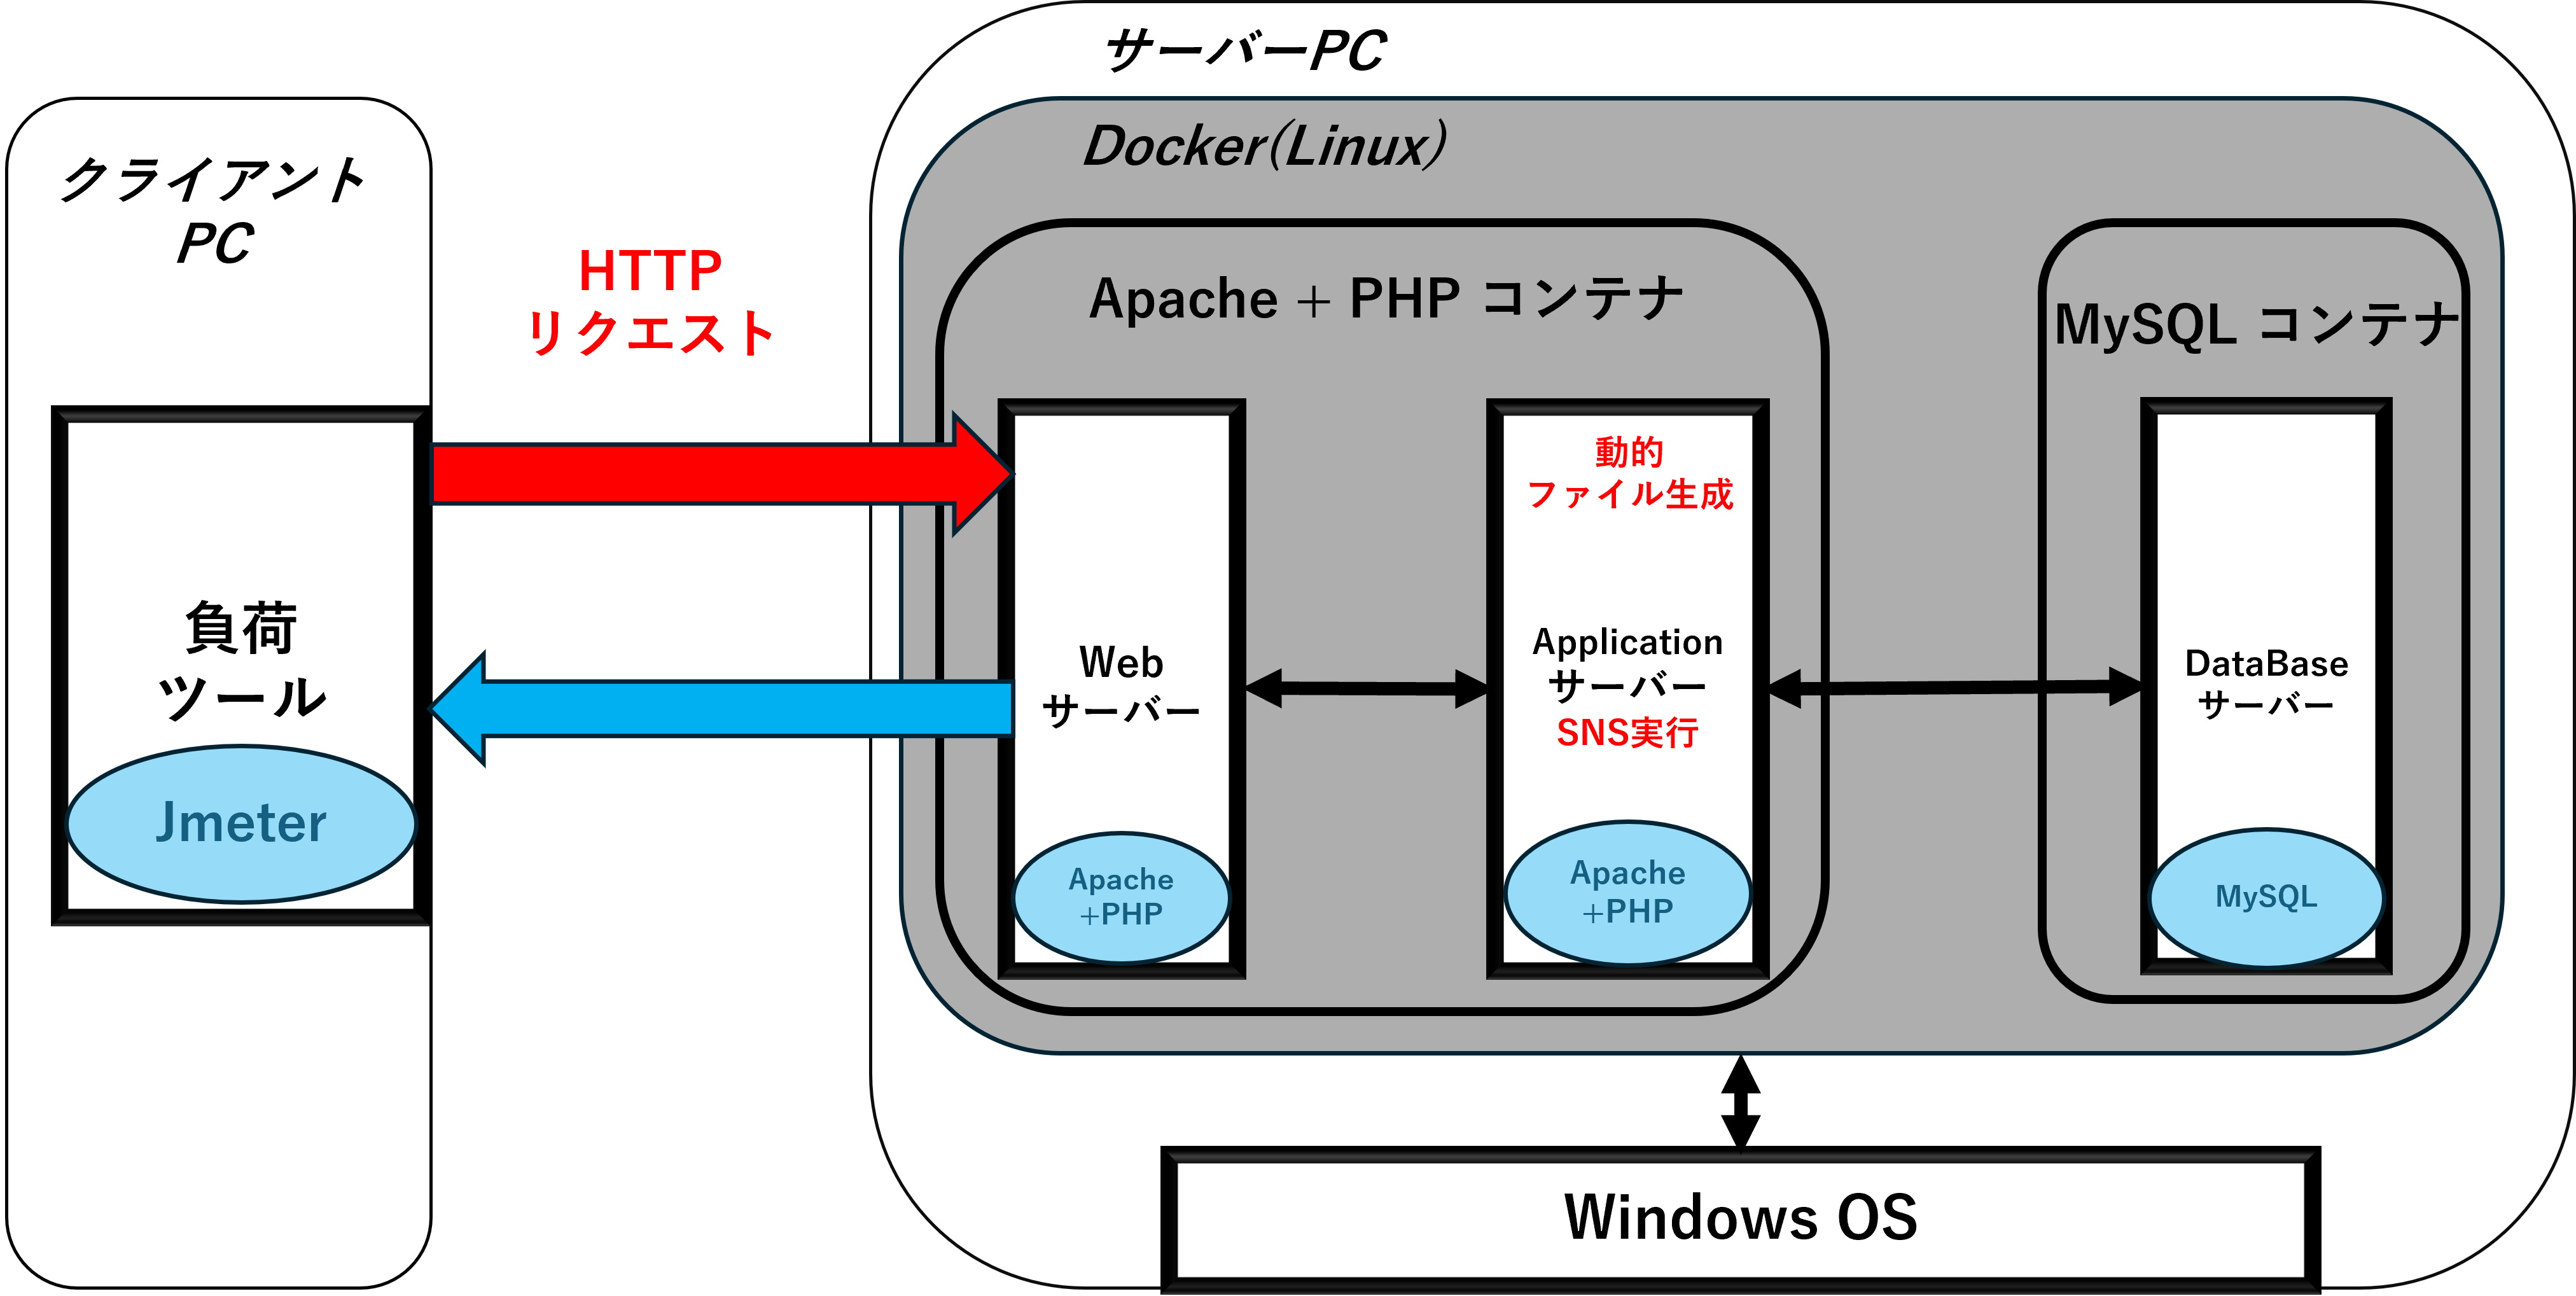
\includegraphics[scale=0.29]{figures/SNS_Docker.png}
  \vspace{-0.6cm}
  \caption{SNS運用環境と負荷ツール}
  \label{fig:1}
\end{figure}
図\ref{fig:1}が実験環境であり,二つのデバイスで構成される.
サーバーPCでは,Dockerにより,Windows OSとOpenPNEの運用環境を隔離している.
また,OpenPNEの環境をDocker上に独立させることで移植性が高く,メトリクスをクリーンに取得できる.
JmeterをインストールしたクライアントPCとは,LANケーブルでつなぐ.
そのため,物理的な接続の影響を受けるリスクがあるが通信関連の外部的な影響は排除できる.

本研究で使用する物理デバイスは以下のとおりである:
\begin{itemize}
  \setlength{\parskip}{0cm} % 段落間
  \setlength{\itemsep}{0cm} % 項目間
  \item サーバーPC:HP Z2 mini G9 workstation desktop PC,13th Gen Intel(R)Core(TM) i9-13900 3.00GHz,RAM:16.00GB,Win11 pro,23H2
  \item クライアントPC:Desktop-7CL98lG,Intel(R) Core(TM)i7-6600U CPU@2.60GHz,RAM:8.00GB,Win10 Enterprise,22H2
\end{itemize}
また,データ収集は以下のように行う:
\begin{itemize}
  \setlength{\parskip}{0cm} % 段落間
  \setlength{\itemsep}{0cm} % 項目間
  \item サーバー側:Docker stats\footnote{https://docs.docker.com/reference/cli/docker/container/stats/}コマンドで取得.\par
  メトリクス:CPU使用率,メモリ使用量(0.5秒毎)
  \item クライアント側:Jmeter\footnote{https://jmeter.apache.org/}で全リクエストを取得.\par
  メトリクス:エラー率
\end{itemize}
\section{実験}
以下の実験において,負荷の大きさは,RPS (Requests Per Second)で表し,Jmeterで設定する.
0h~1hでは10,000スレッドを立ち上げ,1h~25hをシナリオ毎の負荷期間とする.
これらに加え,本研究では,Torquatoらの2018年の研究を参考にし監視期間を考え,\ref{subsec:load1}節,\ref{subsec:load2}節では25h~27hに監視期間を追加し,10RPSの負荷を与えメトリクスを監視する.
% 2018年に,ストレス期間,待期期間,若化期間のそれぞれでリソースの監視を行った研究を参考にし,本研究では監視期間というものを考える.

\subsection{本研究の性能調査}
\label{subsec:limit}
本節では,RPS$=$10,30,50,70で負荷を与え,本環境のサーバーの性能限界を推測する.
\begin{table}[h]
  \centering
  \caption{エラー率とサーバーの性能限界}
  \label{tab:rps}
  \begin{tabular}{ccccc}
    \hline \hline
    負荷 [RPS] & 10 & 30 & 50 & 70 \\ \hline
    エラー率 [\%] & 0.87 & 56.51 & 72.75 & 80.20 \\ \hline
    性能限界 [RPS] & 9.91 & 13.5 & 13.63 & 15.33 \\ \hline
  \end{tabular}
\end{table}

表\ref{tab:rps}は,エラー率および結果から推定できるサーバーの性能限界を示したものである.
性能限界は,1秒間に正しく処理できるリクエスト数だと仮定し,性能限界$=$与えた負荷$×$リクエスト成功率(100$-$エラー率)$/$100の計算により得られたものである。
この結果から,本環境の性能限界は12~15RPS程度であると推測する.

\subsection{シナリオ1:一定負荷}\label{subsec:load1}
\ref{subsec:limit}節の結果より,RPS$=$5,10,15で試行する.
現実において,定常的な状況と対応する.
三つの負荷シナリオについて,1h~25hの負荷期間における全メトリクスは,Mann-Kendall検定\cite{Mann1945Nonparametric}により帰無仮説が否定された.
また,Senの傾き推定\cite{Sen1968Estimates}により傾き$E$の推定値は,0.00005~0.0035の範囲と非常に小さいものの,正の値を示し,ソフトウェアエージングのリスクが発見された.
ただし,検定の対象からは,スレッド立ち上げの影響が残る負荷期間の最初の15分を除く.

\subsection{シナリオ2:増加負荷(監視期間2h)}
\label{subsec:load2}

\ref{subsec:limit}節の結果より,推測した性能限界の範囲内で増加変動を行い,現実における注目度が高まる状況を想定する.
具体的には,1h~25hにかけて,1RPSから15RPSまで線形に負荷を増加させる.
対照実験である\ref{subsec:load1}節の結果と比較し,監視期間における各メトリクスの変動に着目する.
\vspace{0.1cm}
\begin{figure}[h]
  \centering
  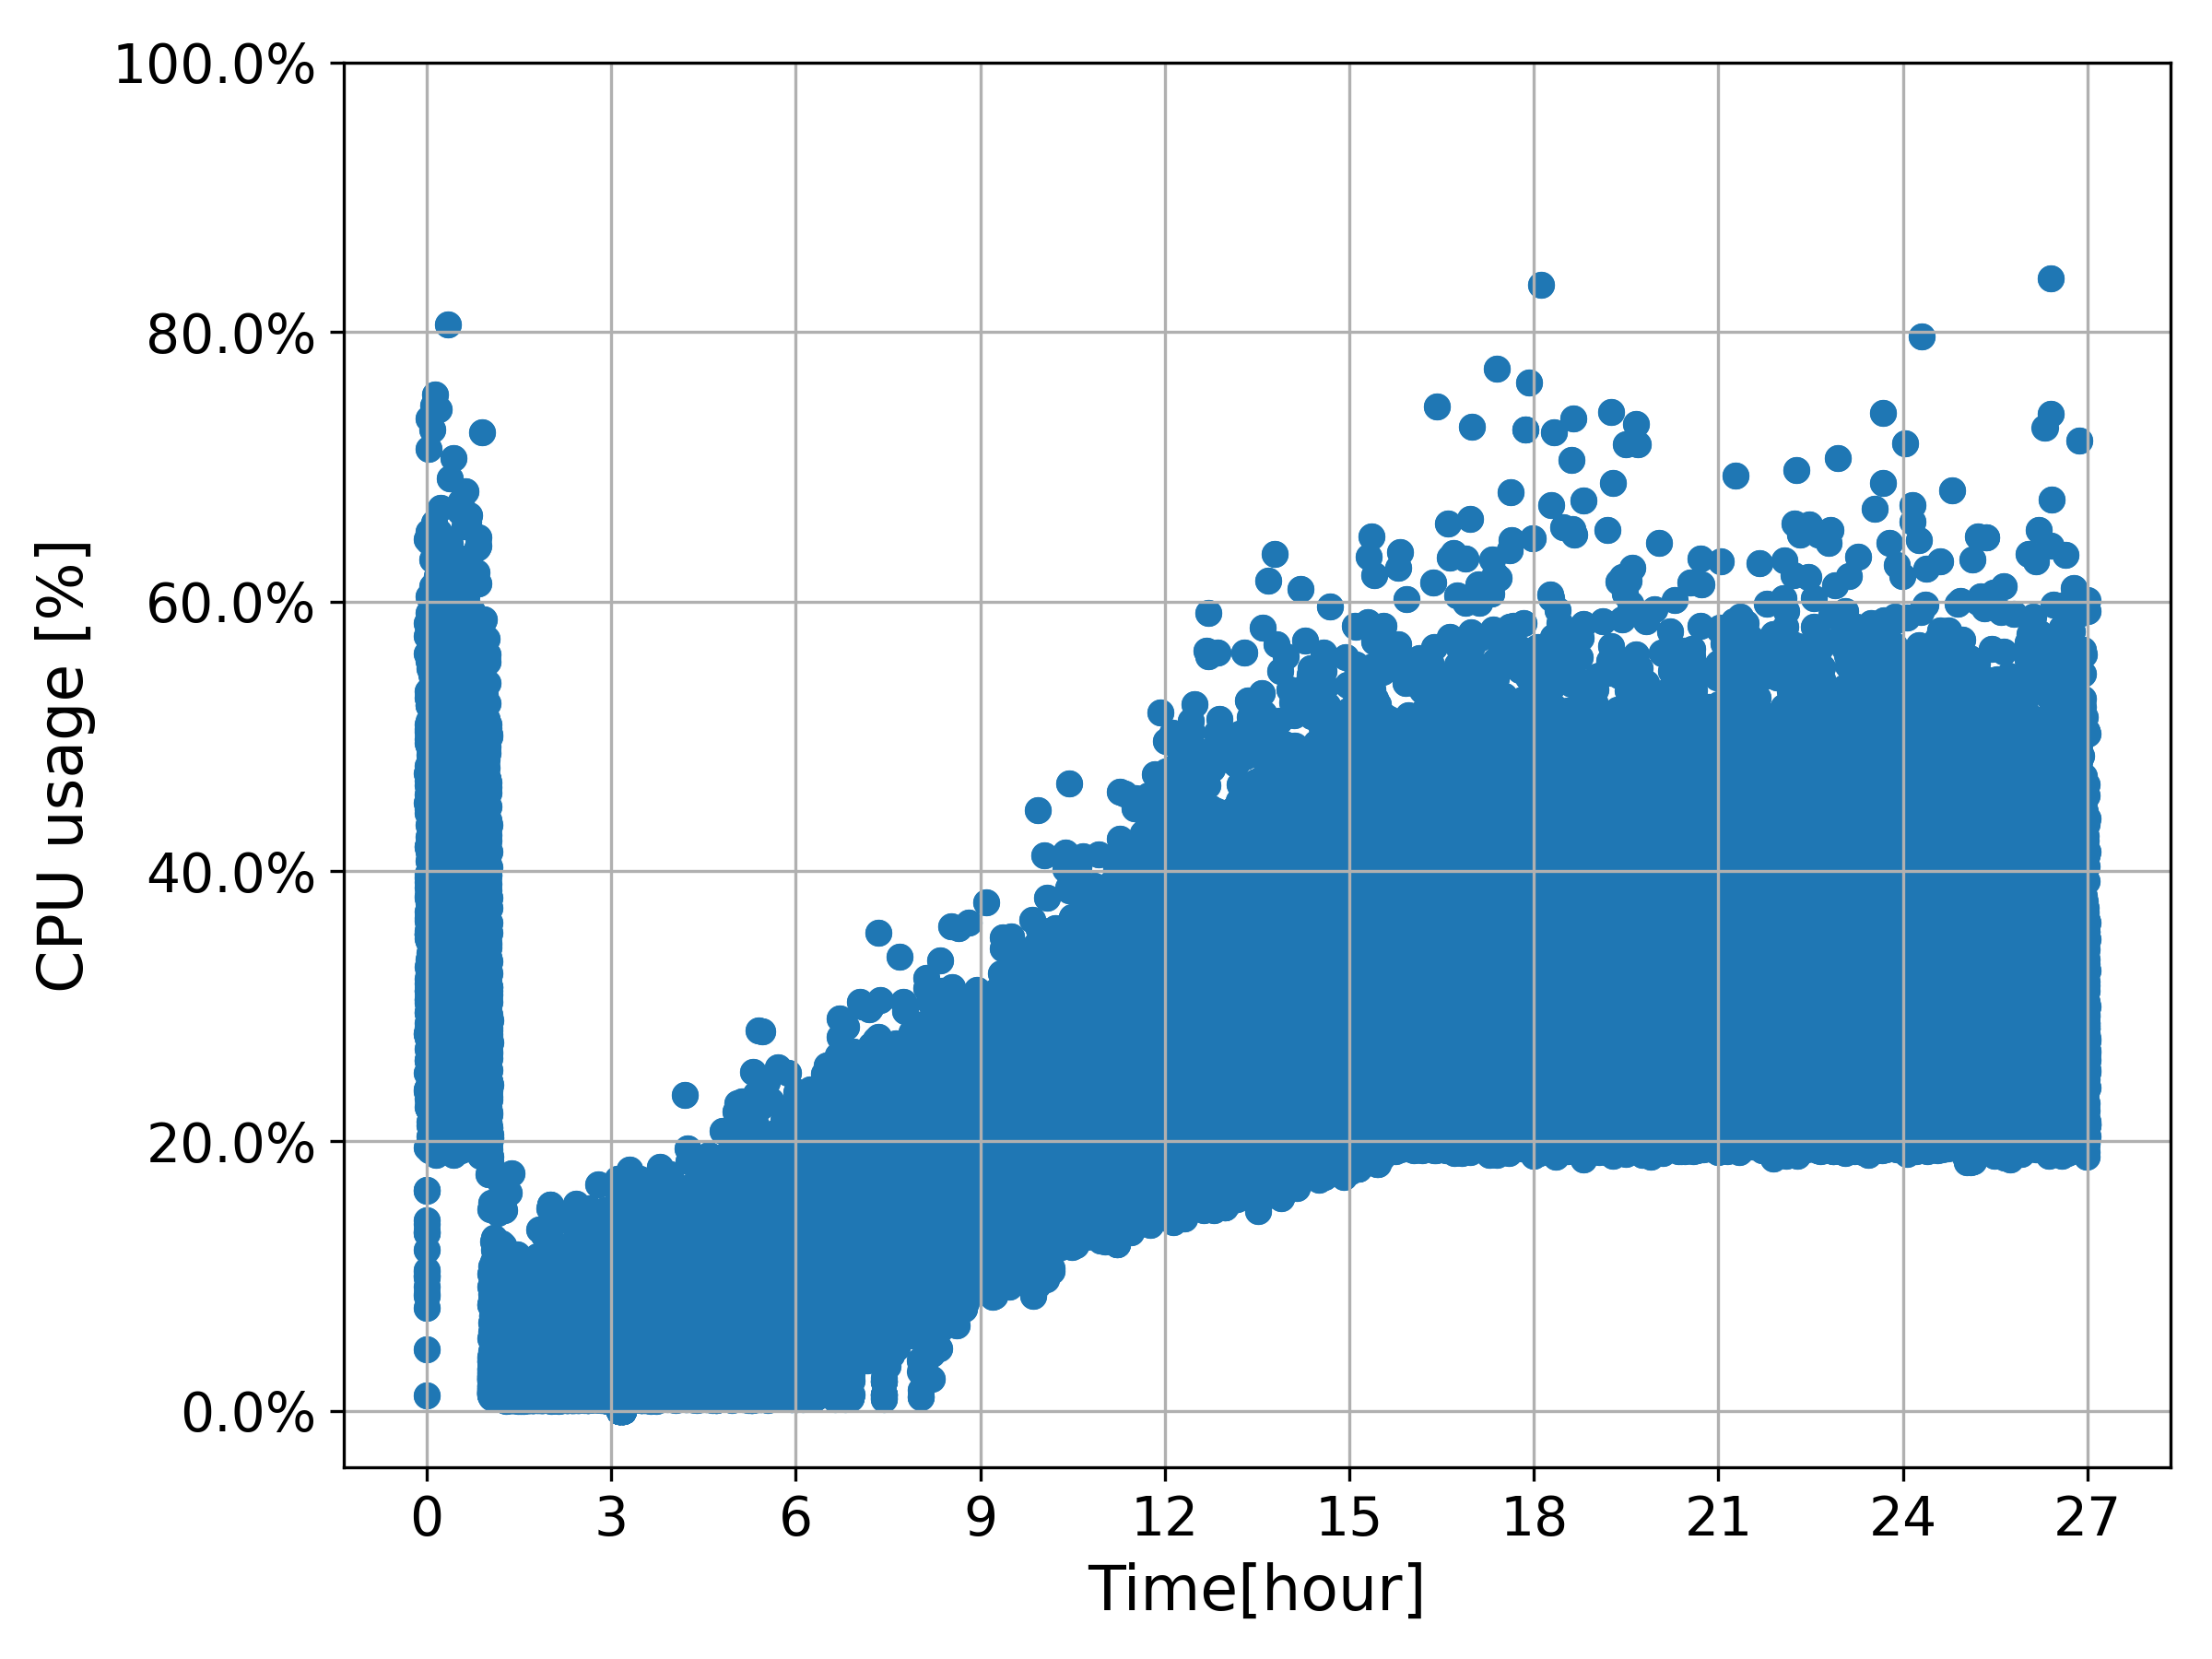
\includegraphics[width=4.3cm]{figures/8core_1_15rps_increase_cpu.png}
  \vspace{-0.5cm}
  \caption{CPU使用率}
  \label{f1}
\end{figure}
\vspace{-0.5cm}
\begin{figure}[h]
  \centering
  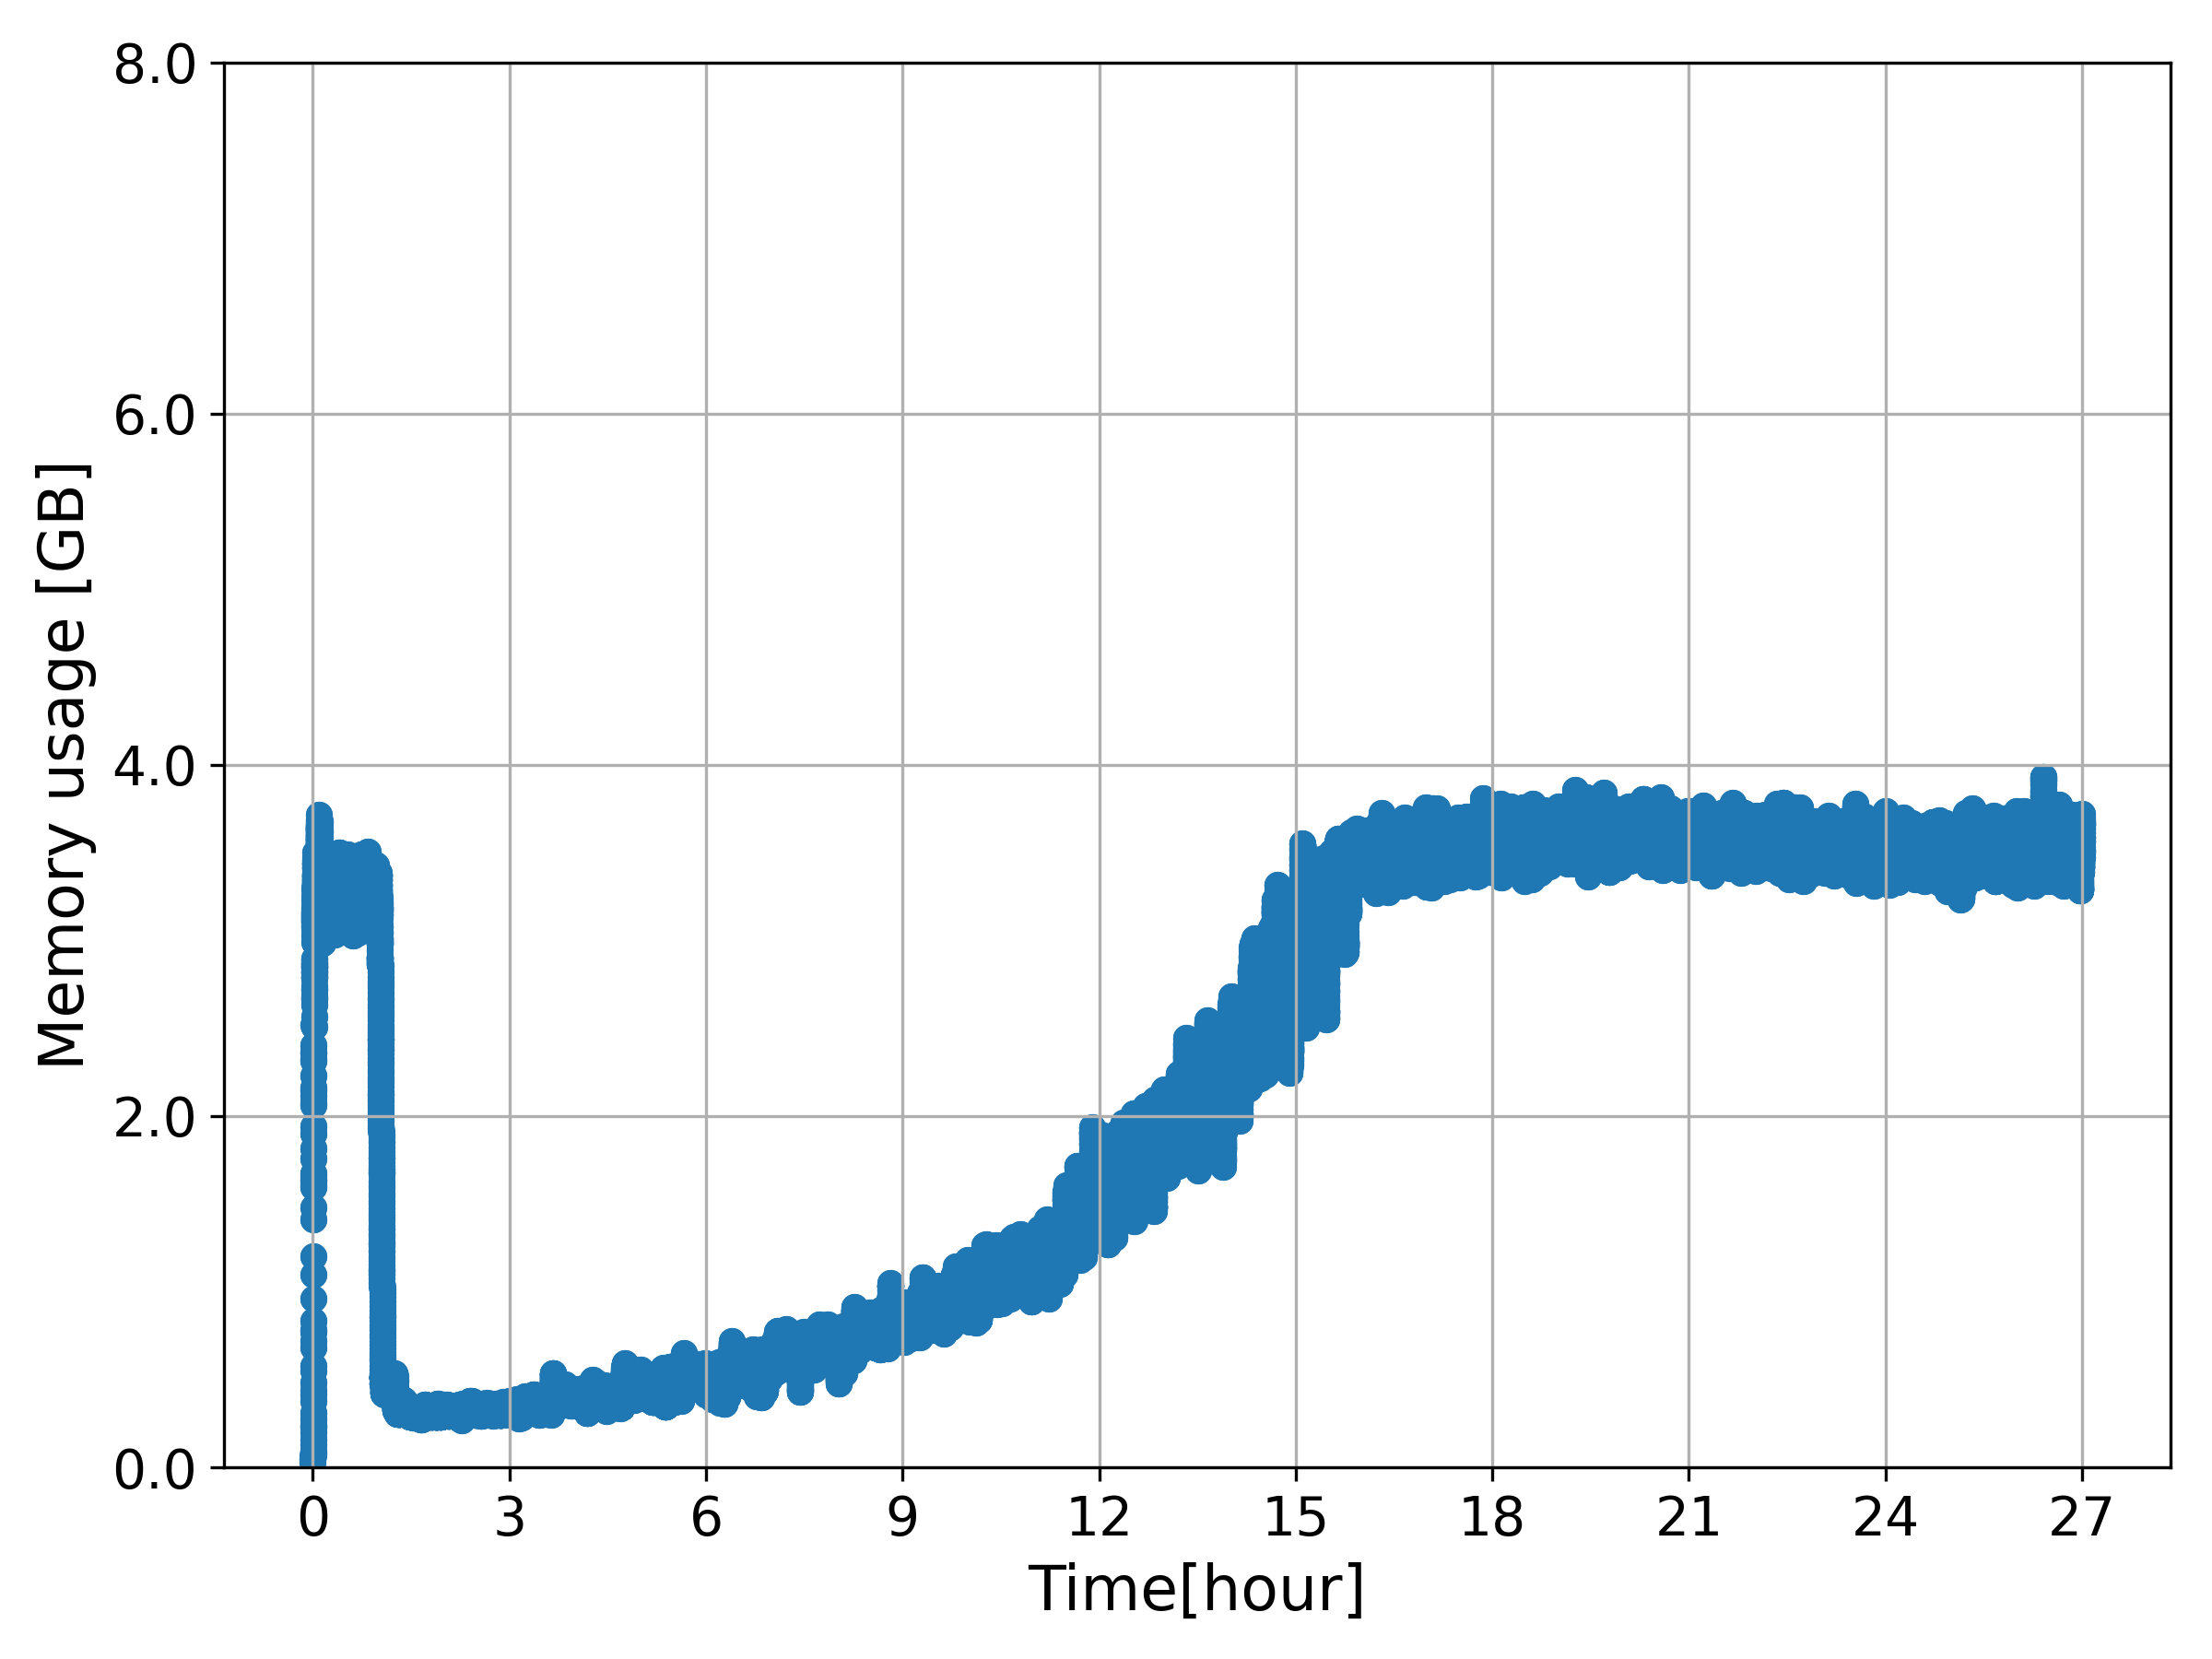
\includegraphics[width=4.3cm]{figures/8core_1_15rps_increase_mem.png}
  \vspace{-0.5cm}
  \caption{メモリ使用量}
  \label{f2}
\end{figure}
\begin{figure}[h]
  \centering
  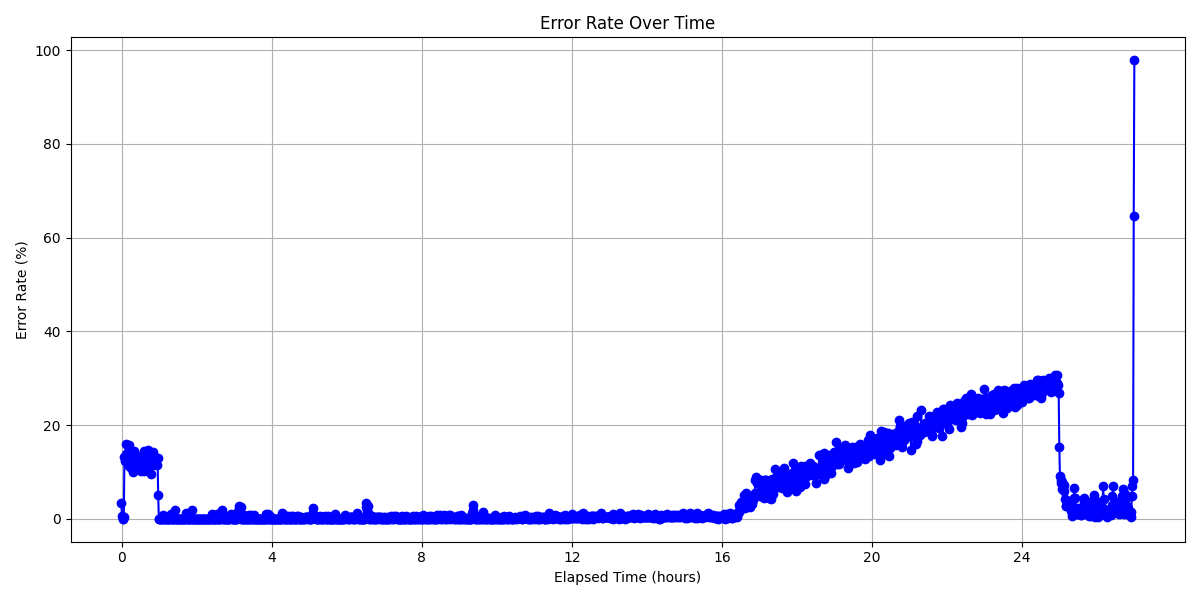
\includegraphics[width=4.7cm]{figures/8core_1_15rps_error_rate.png}
  \vspace{-0.5cm}
  \caption{エラー率}
  \label{f3}
\end{figure}
\vspace{-0.4cm}

図\ref{f1},\ref{f2},\ref{f3}は,増加負荷における各メトリクスの時系列変化である.
スレッド立ち上げ期間は負荷の大きさから各メトリクスが比較的高い値を示している.
増加負荷の期間については,負荷の増加に伴い,全メトリクスが増加していることが分かる.
特に,エラー率については,負荷が10RPS程度に至る16時間ごろから極端に増加しており,推測した性能限界よりも低い負荷の段階でエラーを生じた.
一方で,他二つのメトリクスについては,同時間帯までは増加傾向にあったが,それ以降極端な増加は少なくとも見られない.
これまでの\ref{subsec:limit}や\ref{subsec:load1}節の結果と併せて考えると,メモリ使用量がCPU使用率よりも先に制限に達したことで,エラー率が上昇し始めたと考察する.
ただし,この制限は本研究における環境設定の不備だと考えられる.
具体的には,コンテナに割り当てたメモリは16GB,CPUは8コアであるが,前者は25\%以下,後者は20\%~80\%程度の使用率であるにも関わらず,エラーを生じている.\par
% ここの考察については,卒論では書く
% ことを考えると,メモリ使用の設定に問題があると考えられる.
% この主な原因は,phpのmpm\_eventモジュールが並列処理に不適な環境であることだと考えられる.
また,\ref{subsec:load1}節の結果と比較すると,メモリ使用率,CPU使用率に関しては,負荷期間による監視期間のメトリクスの変動への影響は見られなかった.
% 一方で,エラー率に関しては,その直前の負荷の程度の影響を受ける可能性があると考察する.
% これは,増加負荷と\ref{subsec:load1}節のRPS$=$15の場合を比較すると,視覚的に似た変動をしていたためである.
% ,RPS=5,10の場合と異なり
\section{結論と今後の展望}
本研究では,比較的シンプルなSNSの設定で行い,サーバーの性能限界の推測および比較的低い一定負荷においてもソフトウェアエージングのリスクがあることを発見した.
一方で,増加負荷による各メトリクスの影響は発見できなかった.
今後は,より高度な拡張機能を追加し適切な設定を整えたうえで,ここで得られた知見の検定を行うことが課題である.
近年では,SNSだけでなく,多くのWebサーバーは,クラウド環境に用意されている.
そのため,今後OpenPNEをクラウド環境にデプロイするなどして,大規模でより現実的な負荷テストを行うことが望ましいと言える.
% また,本研究ではソフトウェア若化手法についての検討を行っていない.
% 再起動やガベージコレクションの管理などの代表的な若化手法を,いつ実行すべきかを検討する必要がある.


%%%%%%%%% ここから参考文献 %%%%%%%%%%%%%%%%%%%%%%%
\begin{thebibliography}{5}
  \setlength\itemsep{0.1zh}%←ここの数値を調整(行間のつまり具合)
  \setlength\baselineskip{8pt}
  \textwidth 5pt
  \vskip\baselineskip
  \setlength\baselineskip{4pt}%←ここの数値を調整(追加)(文字の大きさ)
  % \bibitem{Adams1984Optimizing}
  % Adams, N.Edward, “Optimizing Preventive Service of Software Products,” IBM Journal of Research and Development, vol. 28, no. 1, pp. 2-14, 1984.

  % \bibitem{Parnas1994Software}
  % D.L.Parnas, “Proceedings of the 16th International Conference on Software Engineering (ICSE1994),” Software aging, pp. 279-287, 1994.

  % \bibitem{Huang1995Software}
  % Y.Huang, C.Kintala, N.Kolettis and N.D.Fulton, “Software Rejuvenation: Analysis, Module and Applications,” 25th International Symposium on Fault-Tolerant Computing(FTCS1995), pp. 381-390, 1995.

  \bibitem{Dohi2020Handbook}
  T.Dohi, K.Trivedi and A.Avritzer, “Handbook of Software Aging and Rejuvenation,” WORLD SCIENTIFIC, pp. 73-90, 2020.

  \bibitem{Torquato2018SWAREa}
  M.Torquato, Araujo, Matheus, Jean, I.M.Umesh, and P.Maciel, “SWARE: A Methodology for Software Aging and Rejuvenation Experiments,” Journal of Information Systems Engineering \& Management, vol. 3, 2018.

  \bibitem{Mann1945Nonparametric}
  H.B.Mann, “Nonparametric Tests Against Trend,” Econometrica, vol. 13, no. 3, pp. 245-259, 1945.

  \bibitem{Sen1968Estimates}
  P.Sen, “Estimates of the Regression Coefficient Based on Kendall's Tau,” Journal of the American Statistical Association, vol. 63, no. 324, pp. 1379-1389, 1968.

\end{thebibliography}
%%%%%%%%%%%%%%%%%%%%%%%%%%%%%%%%%%%%%%%%%%%%%%%%%%
\end{document}